\chapter{PBS Finder Screen Shots}\label{appendix:screenshots}

\begin{figure}[H]
  \begin{center}
    \leavevmode
    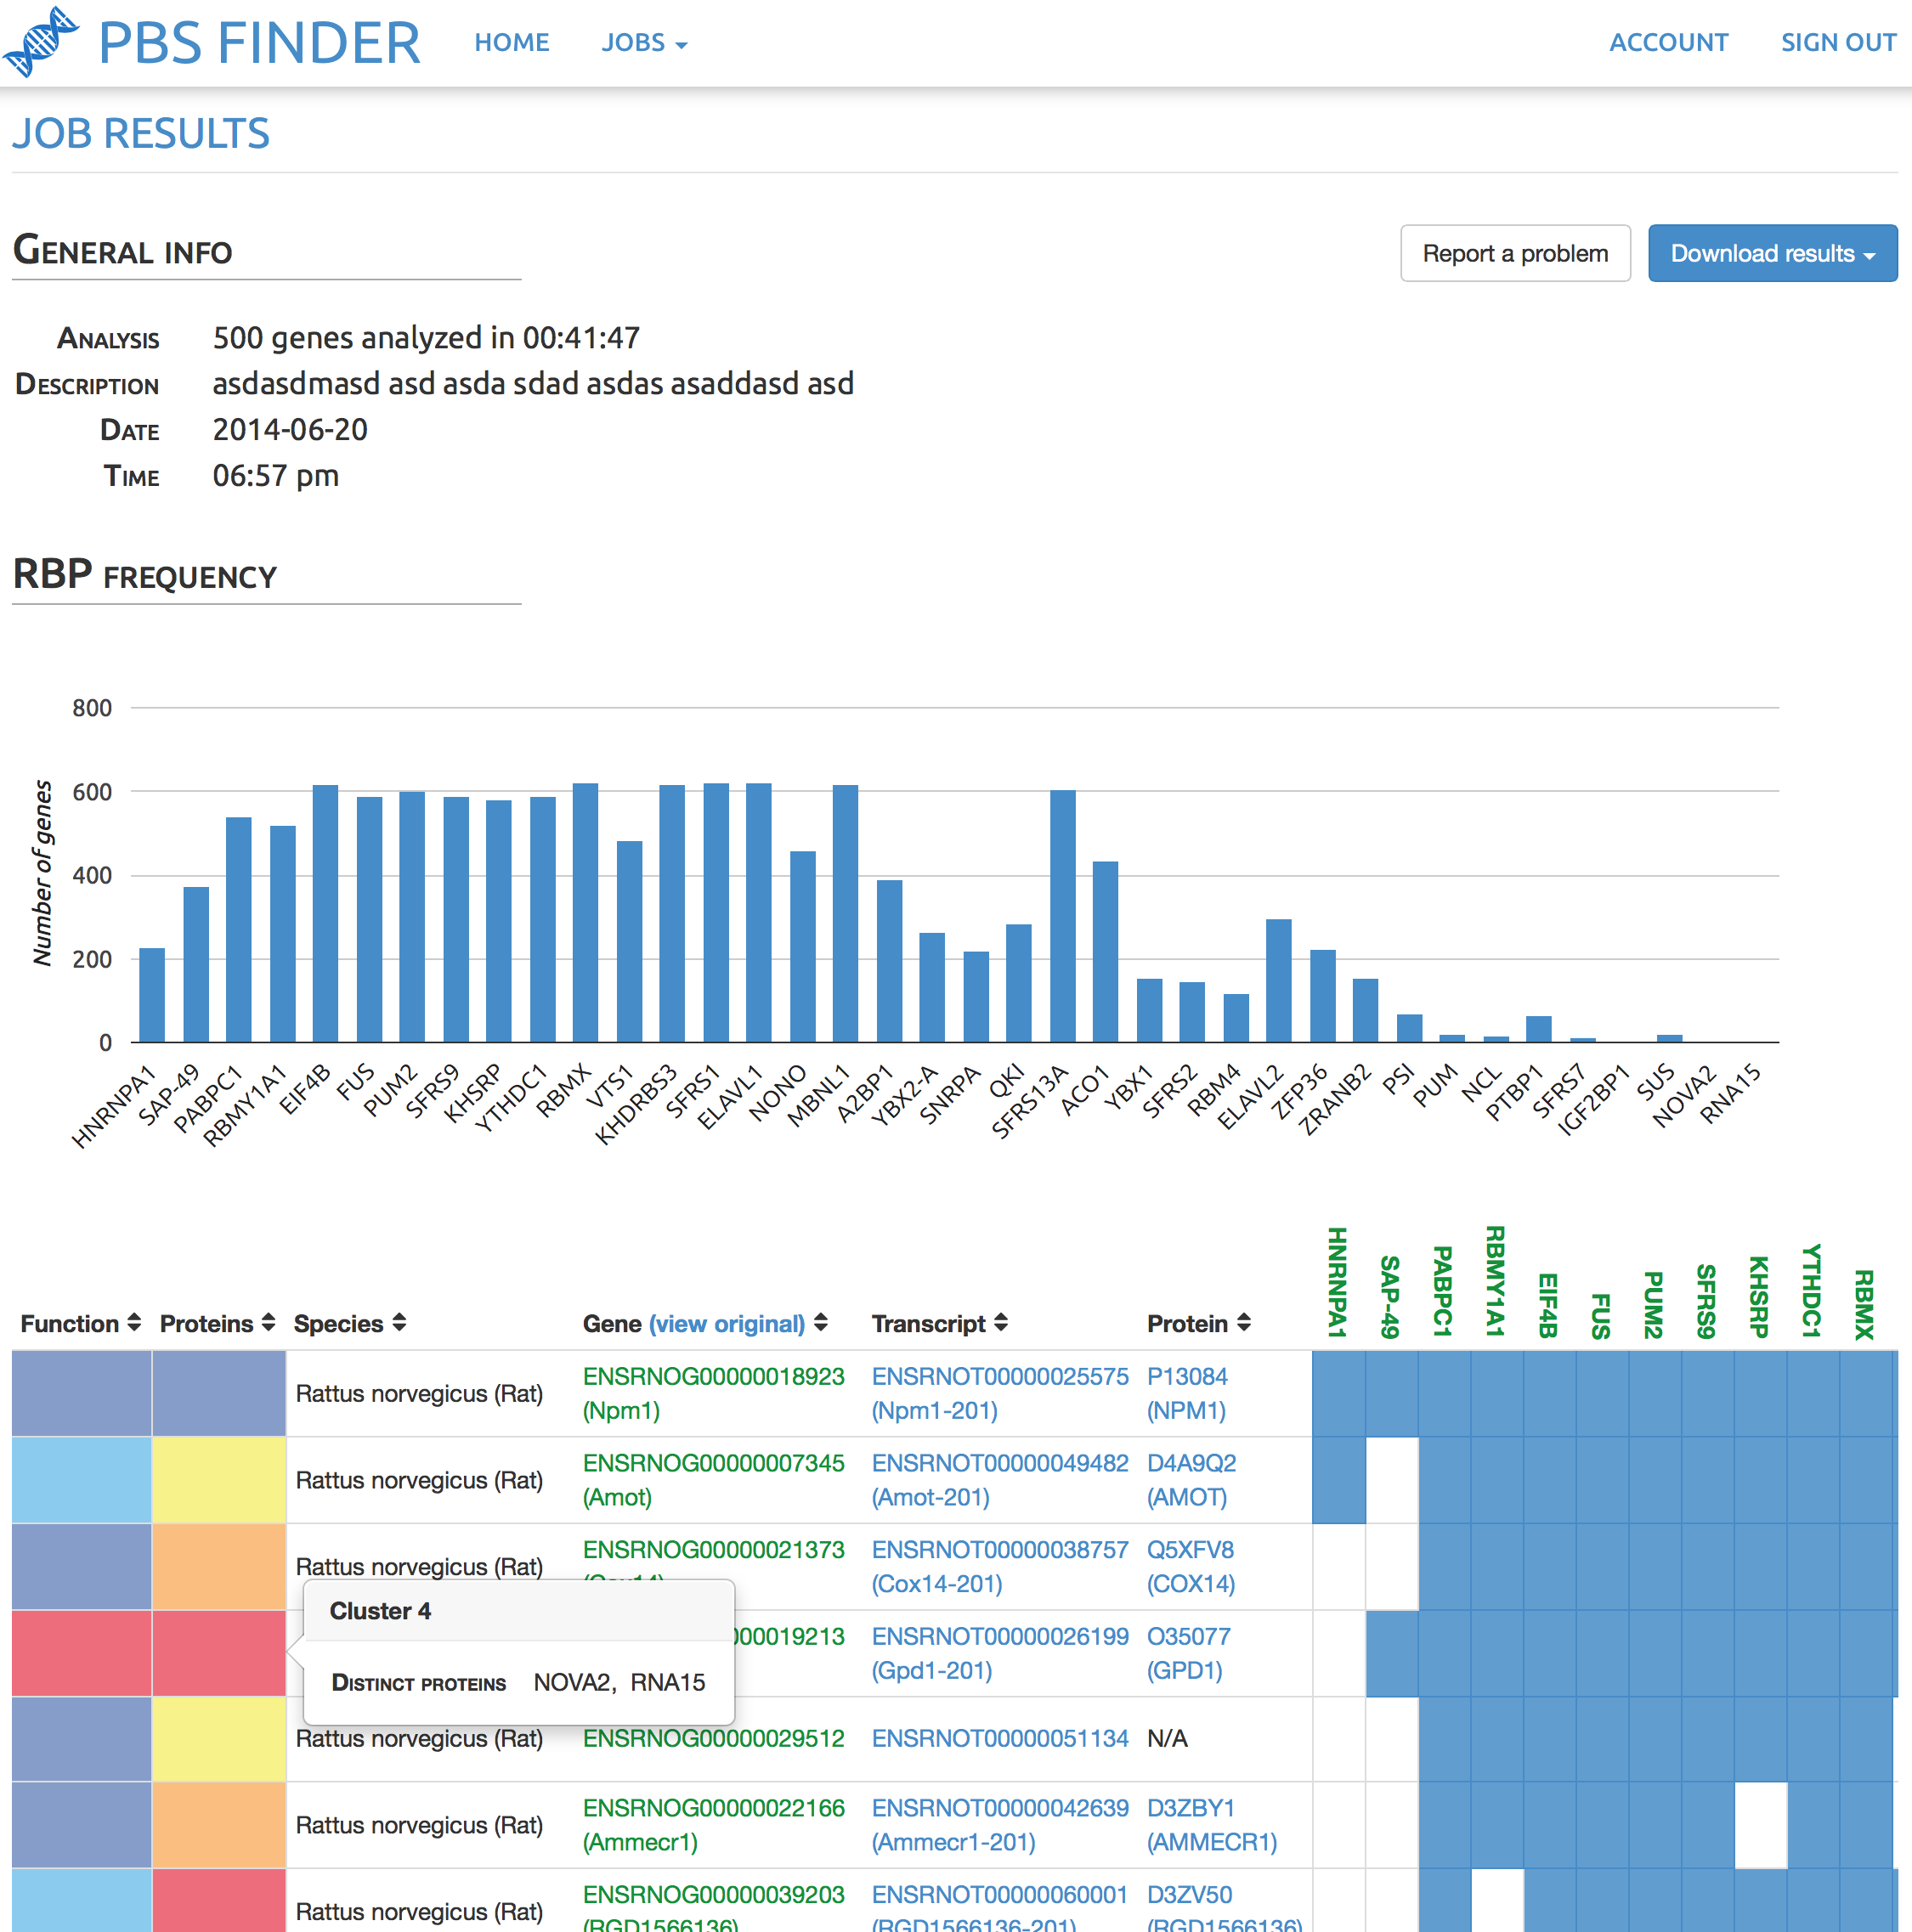
\includegraphics[width=\textwidth]{job_view}
    \caption[Job view example]{
      Job view example, also known as main view. It is comprised by three main
      components: general information (which includes data download); RBP
      frequency histogram; and RNA binding protein matching table.
    }
    \label{fig:job_view}
  \end{center}
\end{figure}

\begin{figure}[!htb]
  \begin{center}
    \leavevmode
    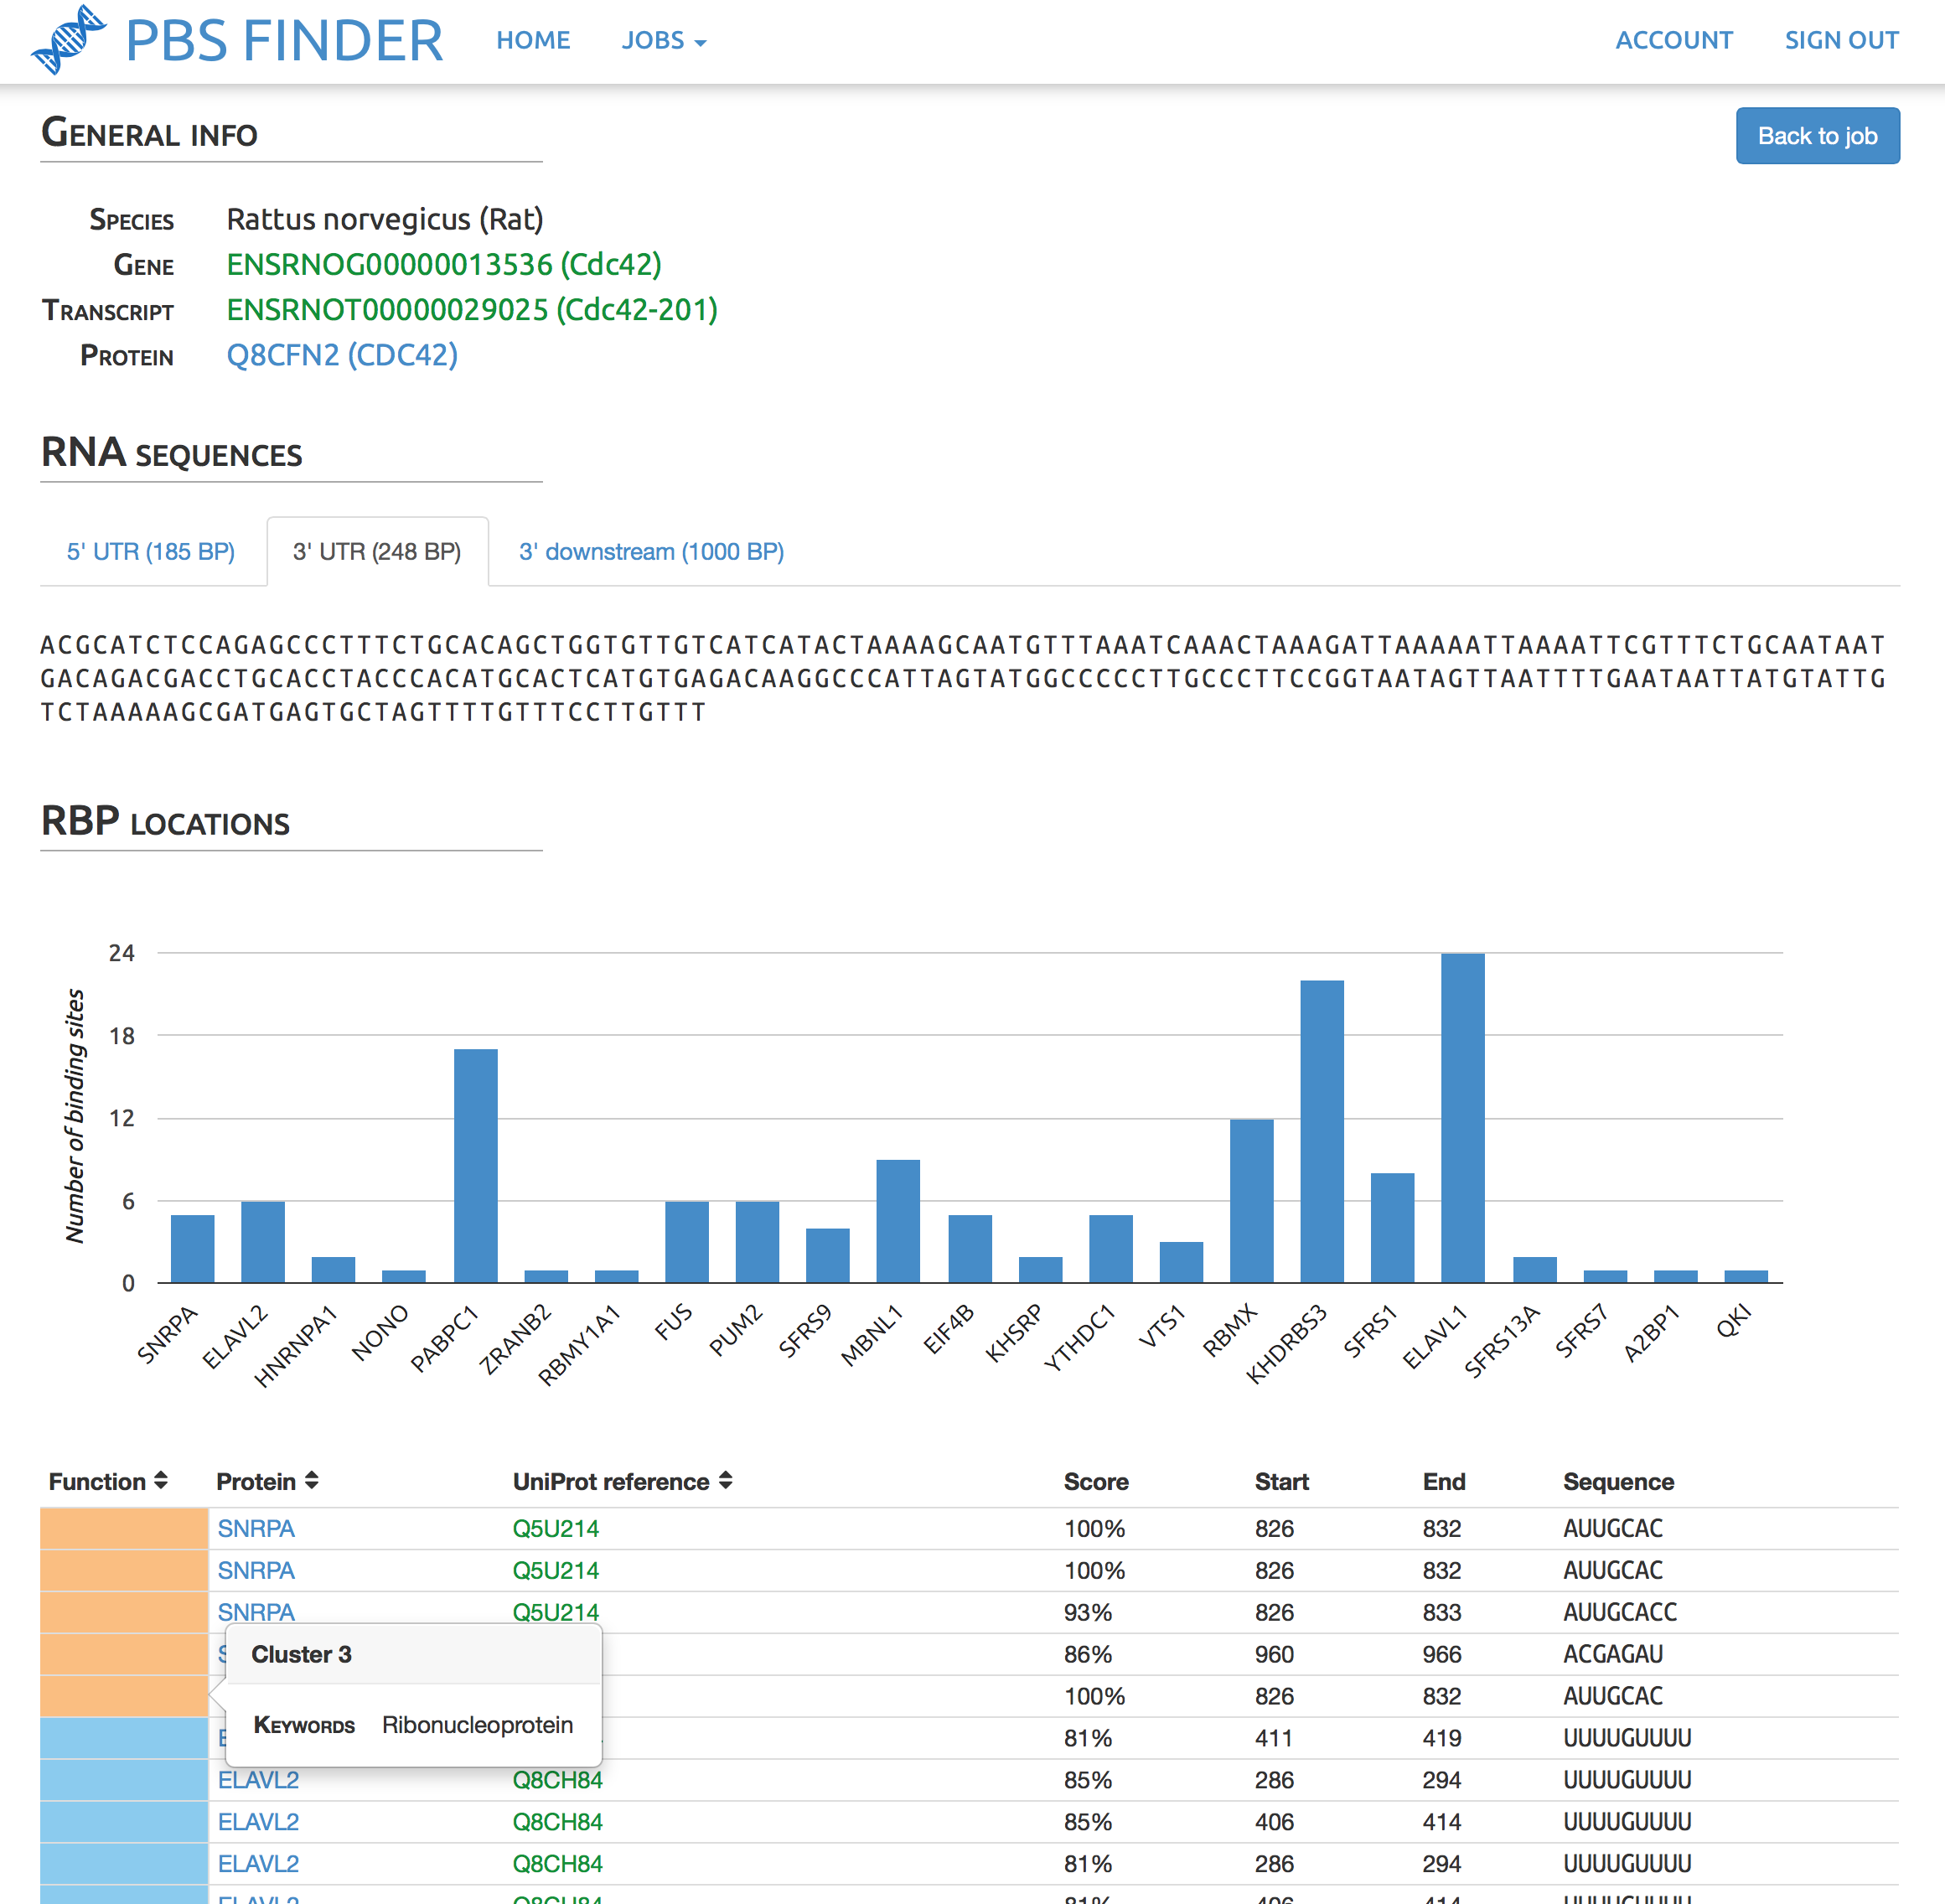
\includegraphics[width=\textwidth]{trans_view}
    \caption[Transcript view example]{
      Transcript view example. It contains four main areas: general information
      about the transcript; RNA sequences (5’UTR, 3’UTR and 3’UTR downstream are
      shown depending on availability); RBP locations histogram; and RBP
      location table (including clustering results and match sequences).
    }
    \label{fig:trans_view}
  \end{center}
\end{figure}

\begin{figure}[!htb]
  \begin{center}
    \leavevmode
    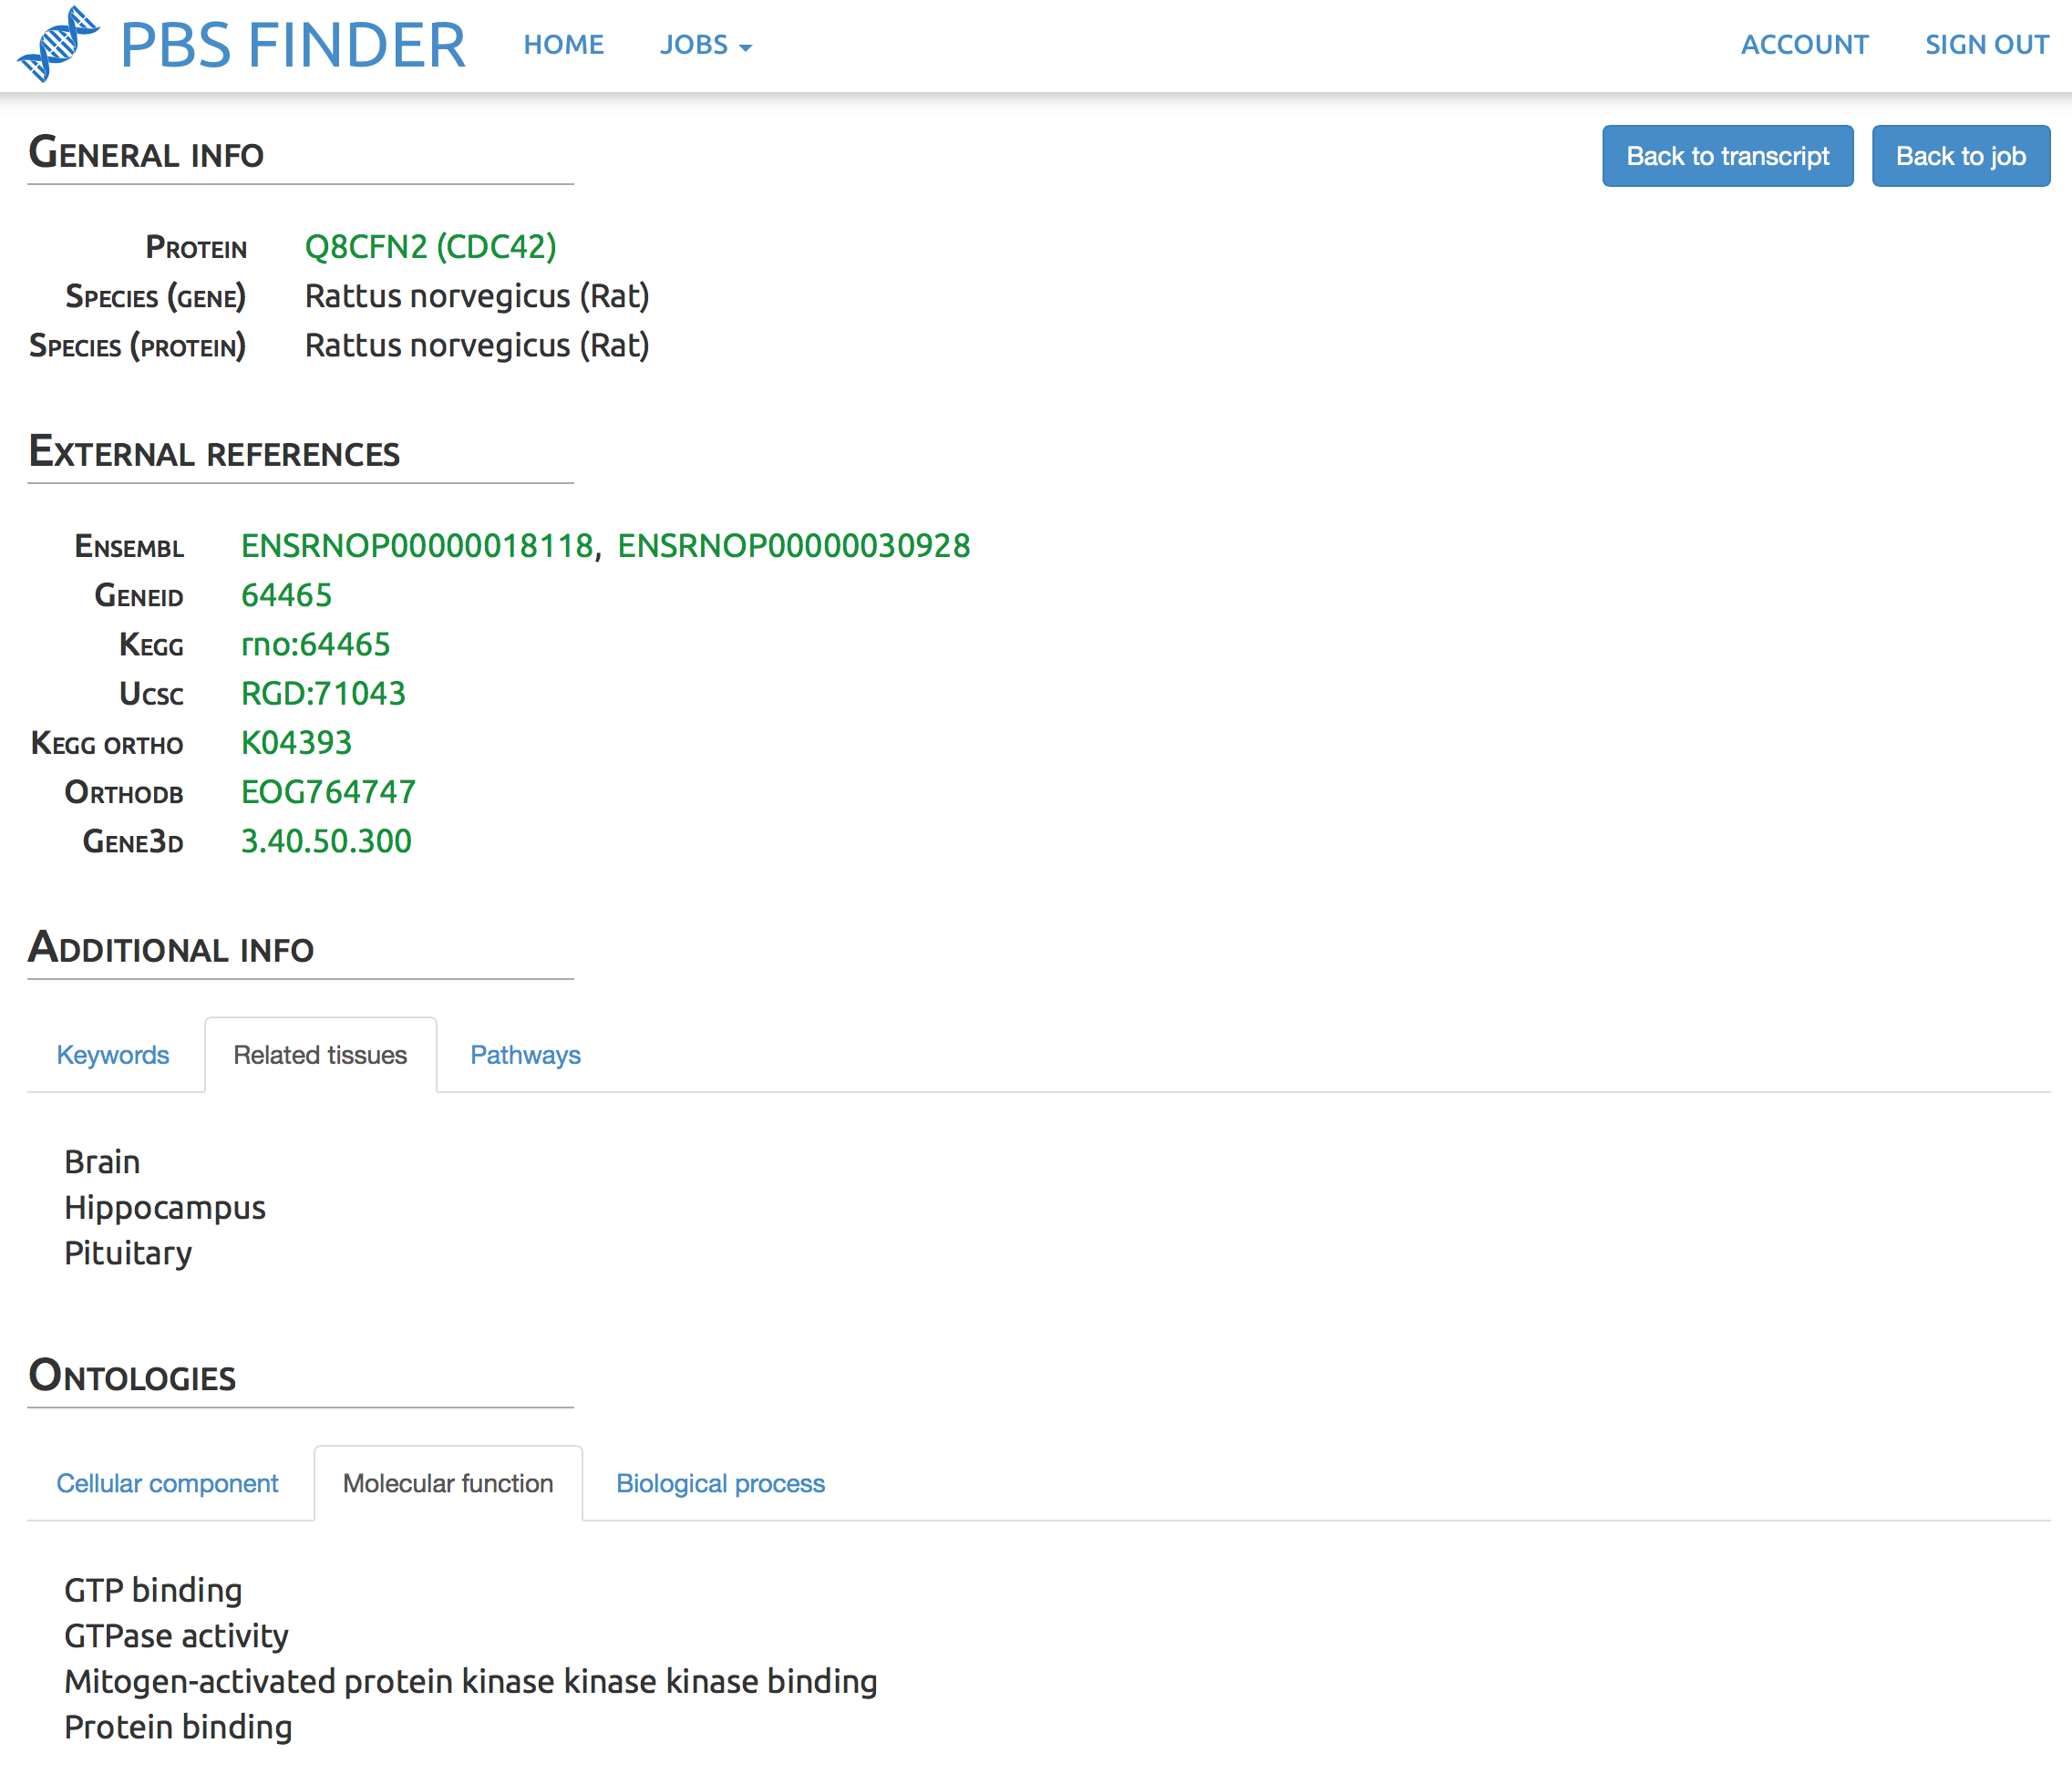
\includegraphics[width=\textwidth]{prot_view}
    \caption[Protein view example]{
      Protein view example, containing four relevant areas: general information
      about the protein; links to other web platforms with relevant information
      about the protein (note that some of those platforms might not contain
      information about a particular protein, and therefore no links can be
      shown); additional info, including keywords, related tissues and pathways
      in which the protein is expressed; and lastly, information about the
      protein's ontologies, including cellular components, molecular functions
      and biological processes.
    }
    \label{fig:prot_view}
  \end{center}
\end{figure}


